\section{Design}
\label{sec:design}

In this section, we describe the design of \ac{name}. We begin with an overview
of \ac{name}'s design. We then describe in detail the two main components of
\ac{name}:
\begin{inparaenum}[(1)]
\item a mechanism to signal which domains have deployed \ac{https}, and
\item a mechanism to enable the verification of multiple certificate chains.
\end{inparaenum}
We conclude the section with a description of how these components enable the
bootstrapping of more advanced policies \steve{cite ARPKI, etc.\@ here?}

\subsection{Overview}
\label{sec:design:overview}

\begin{figure*}
  \centering
  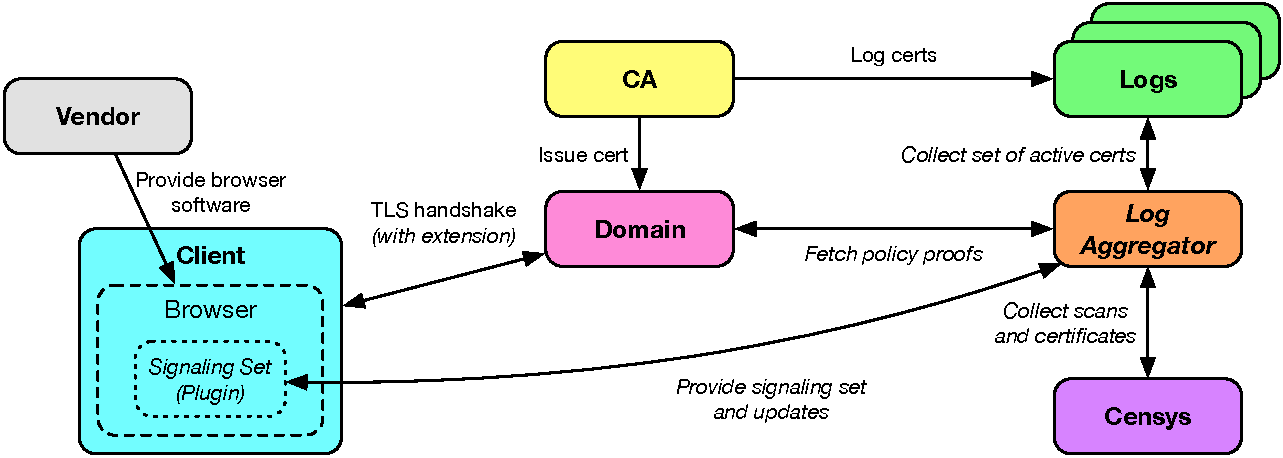
\includegraphics[width=\linewidth]{fig/overview2}
  \caption{Overview of \ac{name} architecture (log auditors and monitors not
  shown). Dotted lines denote the browser and its components, and italic text
denotes new entities or actions in \ac{name}.}
  \label{fig:overview}
\end{figure*}


% What are CAPS's goals and what must it do to achieve those goals?
\ac{name} aims to smoothly transition the current \ac{pki} during the deployment
of a \ac{pki} improvement or a new \ac{pki} (hereafter simply referred to as the
\emph{improved \ac{pki}}). During this deployment process, \ac{name} must
\begin{inparaenum}[(1)]
\item ensure that clients and domains that support the improved \ac{pki} use
  this \ac{pki} when negotiating encrypted connections, and
\item protect public keys in the improved \ac{pki} against the concerted
  misbehavior by $n$ \acp{ca}, where each domain can choose a desired
  nonnegative value of $n$.
\end{inparaenum}

% Architecture
\autoref{fig:overview} illustrates the \ac{name} architecture and how \ac{name}
achieves the goals stated above. Since \ac{name} begins a transition from the
current Web \ac{pki}, it necessarily includes the entities in the current
\ac{pki}:
\begin{compactitem}
\item \emph{Domains} serve webpages to clients. Each domain has a name such as
  \texttt{example.com}. \steve{\endnote{Put somewhere the rules of how domain
  names are differentiated, like www.example.com being a distinct name.}}
\item \emph{\acp{ca}} issue certificates to domains. Each certificate binds a
  set of names to a single public key.
\item \emph{Clients} connect to domains over HTTP or \ac{https}, and in the
  latter case, verify the binding between a domain's name and public key.
\item \emph{Browser/OS vendors} (hereafter simply \emph{vendors}) provide the
  software by which clients connect to domains and verify domains' certificates.
  \steve{\endnote{Possible additional text: Vendors also name a set of root
  \ac{ca} keys.}}
\item \emph{Public logs} maintain a publicly auditable, append-only database of
  certificates.
\end{compactitem}
\ac{name} introduces two new entities:
\begin{compactitem}
\item The \emph{signaling authority} uses data from public logs to construct a
  set of all domains that have deployed \ac{https}.
\item The \emph{log aggregator} uses data from public logs to maintain the
  information that clients use to determine a domain's public key in the
  improved \ac{pki}.
\end{compactitem}
We present the signaling authority and log aggregator as independent entities,
but in \autoref{sec:discussion} we argue why browser vendors and public logs in
the current Web \ac{pki} should respectively take on the responsibilities of
these two entities.

% Procedures from the current PKI
As shown in \autoref{fig:overview}, many of the interactions between entities in
the current \ac{pki} remain the same in \ac{name}. \acp{ca} issue certificates
to domains and log newly-issued certificates as they do in the current \ac{pki}
(with \ac{ct}), clients and domains establish an encrypted communication channel
through the \ac{tls} handshake, and vendors provide clients with browser
software.

% Signaling set overview
To achieve \ac{name}'s goal of signaling which domains have deployed HTTPS, the
signaling authority uses snapshots of the public logs' databases to construct a
\emph{signaling set}, which represents the set of all domains that deploy HTTPS.
The signaling authority builds this set by downloading the set of all currently
valid (i.e., non-expired) certificates from the logs and extracting all domains
named in these certificates. The signaling authority then makes this set, as
well as updates to this set over time, available to client browsers in the form
of a plugin. To minimize the storage and memory overhead of the signaling set,
the signaling authority applies data compression techniques to create a
representation of the signaling set that is space and memory-efficient.

% Policy overview
To achieve \ac{name}'s goal of protecting public keys against $n$ misbehaving
\acp{ca}, the log aggregator uses snapshots of the public logs' databases to
construct a set of \emph{key policies}, which establishes for each
HTTPS-deploying domain one or more public keys to be treated as authoritative in
the improved \ac{pki}. To provide a smooth transition from the current \ac{pki},
\ac{name} uses a simple, intuitive policy to determine a domain's public key in
the improved \ac{pki}: \emph{treat whichever public key is backed by the most
  independent certificate chains\endnote{By \emph{independent} we mean that the
  certificate chains share no public keys except at the leaf.} in the current
\ac{pki} as authoritative in the improved \ac{pki}}.

%Our policy also implies that if $n$ is the
%highest number of observed independent certificate chains for a given domain,
%then \emph{any} public key backed by $n$ chains can be used as that domain's in
%the improved \ac{pki}. Thus, it is possible for a domain to have multiple public
%keys in the improved \ac{pki}.\endnote{In practice, any improved \ac{pki} can
%enforce the use of a single public key by, for example, considering the first
%key backed by $n$ chains as authoritative and using a ``cool-off period'' as in
%AKI~\cite{kim2013accountable}.}


%To move towards \iac{pki} with increased resilience to the compromise of trusted
%parties (i.e., \acp{ca}), we need to prevent \iac{ca} that misissues a
%certificate for a domain from exposing that domain to \iac{mitm} attack. We
%observe that signatures from multiple independent \acp{ca} on a single public
%key can spur greater trust in the key, and therefore we design \ac{name} around
%the idea that domains should be able to obtain and communicate the presence of
%multiple certificates for a single public key. We can then protect domains from
%\ac{mitm} attacks by simply communicating to the client the number of
%certificates to expect. This approach results in simple policies that require
%domain involvement only in rare cases of deliberate misissuance, and allow
%security-conscious domains to ``ratchet up'' their security to their desired
%level.

%\ac{name} leverages \ac{ct}'s infrastructure in its policy mechanism, and
%therefore the two systems have similar architectures, as shown in
%\autoref{fig:overview}. \steve{TODO: add Censys data and an external service or
%browser vendor to the overview figure} \ac{name} assumes a full deployment of
%\ac{ct}, that is, all certificates must be logged for clients to accept them as
%valid. \steve{Beginning in October 2017, Chrome will begin enforcing this
  %requirement for all \ac{https} sites, so this assumption is a reasonable one.}
  %For the purposes of obtaining \acp{sct}, the logging process works just as it
  %does in \ac{ct}. Also as with \ac{ct}, public logs are kept accountable by
  %auditors and monitors, and an external party (Google in the case of \ac{ct})
  %maintains a list of known trusted logs.

%In \ac{name}, however, logs maintain an additional database of certificate
%policies alongside their database of certificates. The logging process also
%triggers changes in this policy database. Domains periodically request the proof
%for their latest policy from the logs and provide both their policy and proof to
%clients during the \ac{tls} handshake. We further describe the details of our
%policy mechanism in \autoref{sec:policy}.

%Client browsers locally maintain a \emph{signal set}, which indicate whether or
%not a given domain has deployed \ac{https}. The browser queries the signal set
%before initiating an HTTP or \ac{https} connection to a site 
%in order to determine
%\begin{inparaenum}
%\item whether or not to establish \iac{https} connection, and
%\item if so, how many certificates to expect.
%\end{inparaenum}
%If the signal set indicates that the domain has deployed \ac{https} but the
%server does not provide a certificate, the browser aborts the connection,
%assuming that an adversary is attempting to mount \iac{tls} stripping attack.

%The signal set is created by using data from the \ac{ct} logs. This data is used
%to construct a list of all DNS names for which a \ac{tls} certificate has been
%observed (either as the main subject or as a subject alternative name). This
%list is then represented using \iac{dafsa} that recognizes the DNS names of
%sites that deploy \ac{https}. By using compression techniques, we compact this
%\ac{dafsa} into a representation that requires little storage. Such a compact
%representation allows us to store the \ac{dafsa} in memory, offering performant
%lookups. We further describe the details of our signal set design in
%\autoref{sec:design:signaling}.

\subsection{Signaling HTTPS Deployment}
\label{sec:design:signaling}

\begin{compactitem}
\item High-level overview of FSA approach \steve{TODO: graphic}
\item Shortcomings of other approaches
  \begin{compactitem}
  \item Bloom filters, filter cascades, probabilistic approaches have FPs/FNs
    and still are large or require global view of all domain names
  \item Standard compression utilities would require the set to be decompressed
    before querying members
  \item Tries only take into account common prefixes
  \end{compactitem}
\item FSA creation
\item FSA compaction techniques
  \begin{compactitem}
  \item Coalescing single-edge paths
  \item Compacting 1:N nodes
  \item Binary representation
  \item Huffman encoding labels
  \item Huffman encoding destinations
  \end{compactitem}
\item Updating the FSA
\end{compactitem}

\subsection{Verifying Multiple Certificate Chains}
\label{sec:design:verifying}

\begin{compactitem}
\item Log aggregation
  \begin{compactitem}
  \item Periodically collect snapshots from logs (similar to a log monitor in
    \ac{ct})
  \item maintain a database containing certificate chains that are valid (i.e.,
    no certificate in the chain has expired)
  \item maintaining a trusted set of root \acp{ca} for certificate chains is not
    necessary, since the logs do this already
  \end{compactitem}
\item Determining the key policy
  \begin{compactitem}
  \item Given a set of currently valid certificate chains for the same public
    key, take the min-cut to find the strength of this key
  \item Consider EV certificates separately from non-EV certificates
  \item Repeat this for all public keys for a domain, thus forming a $(m, n)$
    pair for each key where $m$ is the number of EV certs and $n$ the number of
    non-EV certs
  \item The key policy is $(x, y)$ where $x$ is the maximum of all $m$ values
    observed and $y$ is the maximum of all $n$ values for that specific $m$
    value
  \end{compactitem}
\item Expiration/revocation
\item Update interval
\item Modified handshake
  \begin{compactitem}
  \item Signal through TLS extension
  \item Domain sends multiple chains, proof of key policy (for efficiency)
  \end{compactitem}
\end{compactitem}

\subsection{Bootstrapping Advanced Policies}
\label{sec:design:bootstrapping}

\begin{compactitem}
\item Use keys established by these key policies to bootstrap more advanced
  policies
\item As an example, use PoliCert (since it has a clean separation between
  policy and certificate)
\end{compactitem}
